\section*{Task 1 --- Forecasting Across Heterogeneous Sensors}
All numbers below are copied from the executed full-preset notebook (\texttt{Question\_1/Assignment1.ipynb}, data seed 0, model seed 0, CUDA). Unless stated otherwise, errors are \textbf{validation} RMSE in m/s$^2$. ``Est.'' means established Stations 1--3, and ``S4'' means held-out Station 4.

\subsection*{Response 1A: Predict, measure, and revise the aggregate ordering}
\textbf{Prior, written before Output 1.1.} \emph{Established:} period-routed ridge $>$ Raw Attention $>$ sensor-specific ridge $>$ shared ridge. \emph{S4:} period-routed ridge $>$ Raw Attention $>$ shared ridge (sensor-specific ridge cannot be applied to S4). My reasoning was that period routing conditions on operating pace, which is the quantity that actually changes.

\begin{table}[H]\centering\small
\caption*{Output 1.1 --- validation RMSE (m/s$^2$) by population and product}
\begin{tabular}{lcccc|cccc|r}\toprule
 & \multicolumn{4}{c|}{Established (S1--3)} & \multicolumn{4}{c|}{Held-out S4} & \\
Model & all & A & B & C & all & A & B & C & Params\\\midrule
Shared ridge & 0.767 & 0.805 & 0.854 & 0.621 & 0.876 & 0.909 & 0.982 & 0.713 & 4,608\\
Sensor-specific ridge & 0.768 & 0.804 & 0.852 & 0.630 & n/a & n/a & n/a & n/a & 13,824\\
Period-routed ridge & \textbf{0.166} & \textbf{0.181} & \textbf{0.164} & \textbf{0.152} & \textbf{0.173} & \textbf{0.184} & \textbf{0.182} & \textbf{0.150} & 59,904\\
Raw Attention & 0.466 & 0.452 & 0.502 & 0.442 & 0.679 & 0.731 & 0.617 & 0.685 & 368,368\\\bottomrule
\end{tabular}\end{table}

\textbf{Revised ordering.} \emph{Established:} period-routed ridge (0.166) $>$ Raw Attention (0.466) $>$ shared ridge (0.767) $\approx$ sensor-specific ridge (0.768). \emph{S4:} period-routed ridge (0.173) $>$ Raw Attention (0.679) $>$ shared ridge (0.876). My top two were right. I revise one thing: sensor-specific ridge is \emph{not} better than shared ridge. The two are tied.
\begin{itemize}
\item \textbf{Station identity does not help.} One matrix per station gives the same error as one matrix for all stations (0.768 vs 0.767). Each station runs at every pace, so each per-station matrix faces the same compromise.
\item \textbf{Pace is the right conditioning variable.} Period routing is 2.8$\times$ more accurate than Raw Attention on Est. (0.166 vs 0.466), and 3.9$\times$ on S4 (0.173 vs 0.679). It is also the best model on every product. Its error changes little across products (0.15--0.18), whereas shared ridge ranges from 0.62 to 0.98.
\item \textbf{Generalisation to S4.} Period routing loses only 4\% on S4 (0.166 $\to$ 0.173), because it uses only the period estimated from the context. Raw Attention loses 46\% (0.466 $\to$ 0.679). It has to recover the pace from learned Q/K features, which were fitted only on the mounting and drift of Stations 1--3.
\end{itemize}

\subsection*{Response 1B: Why the rule must depend on context}
\begin{figure}[H]\centering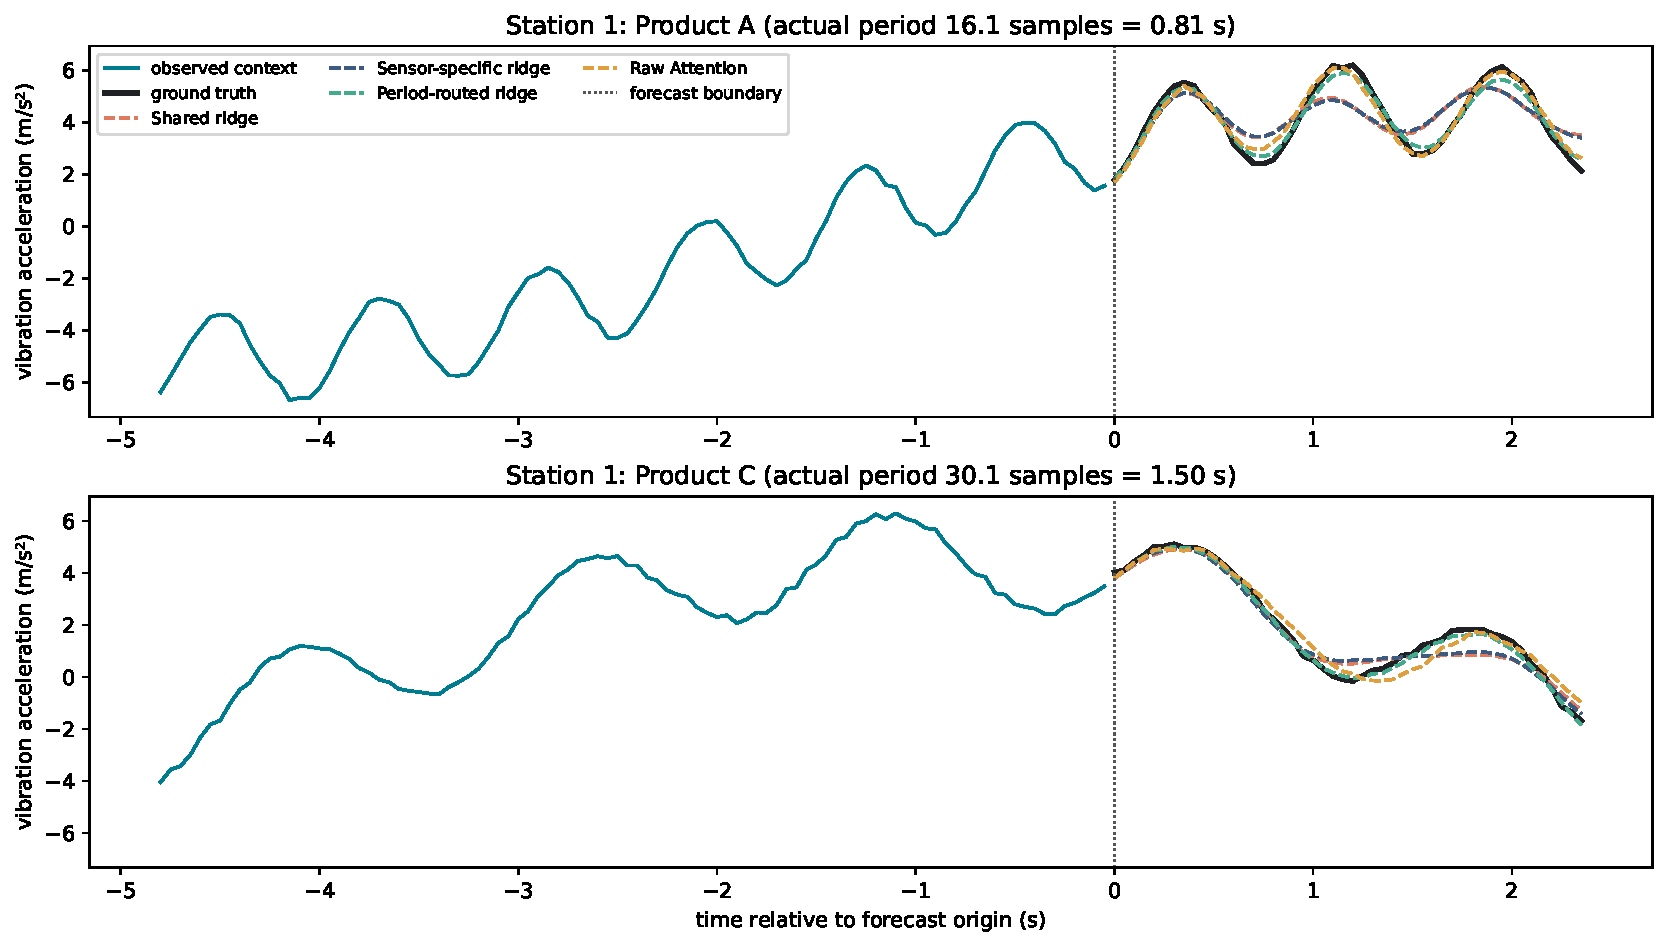
\includegraphics[width=0.9\linewidth]{../Figures/1.2-1.pdf}\caption*{Output 1.2 --- Station 1 under Product A ($P=16.1$) and Product C ($P=30.1$)}\end{figure}
\textbf{The fixed matrix $\hat W$ (Eq.~8) must compromise.} It applies one linear map whatever the pace. The Product A run ($P=16.1$) and the Product C run ($P=30.1$) need different phase advances over the 48-step horizon, but $\hat W$ contains no variable that selects between them. Least squares therefore averages the incompatible continuations. In Output 1.2 the shared-ridge forecast is damped (reduced amplitude), and its peaks drift out of phase with the truth as the lead time grows. The window RMSE shows this: shared ridge scores 0.779 (A) and 0.448 (C), while period-routed ridge scores 0.232 and 0.150.

\begin{figure}[H]\centering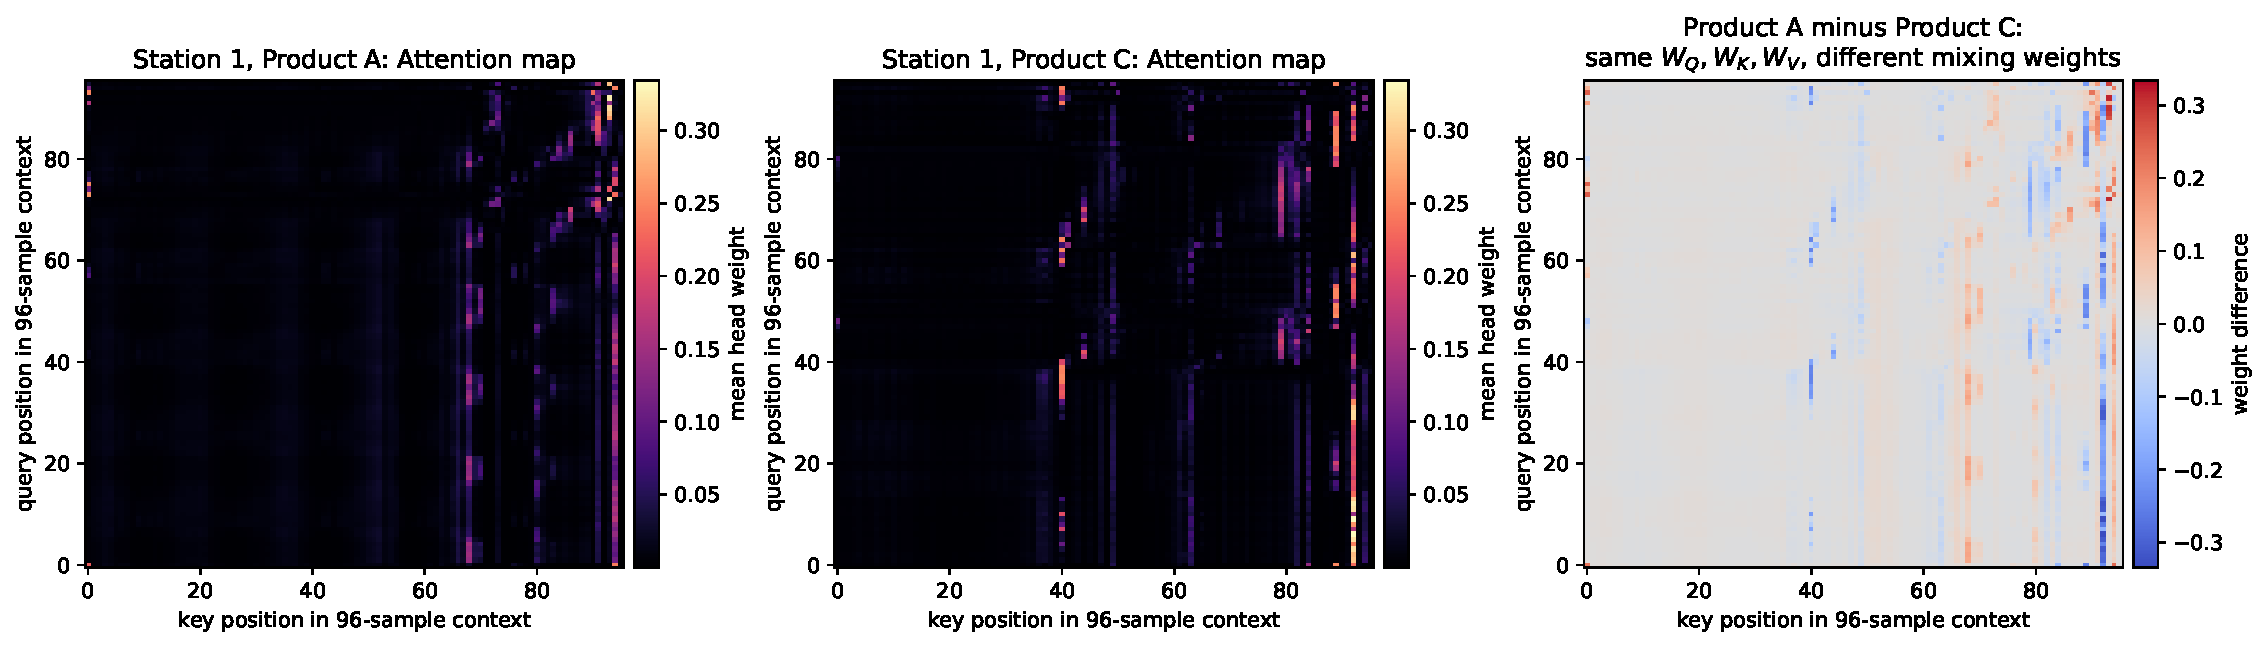
\includegraphics[width=0.9\linewidth]{../Figures/1.3-1.pdf}\caption*{Output 1.3 --- Attention weights for the two contexts and their difference}\end{figure}
\textbf{Attention builds its mixing rule from the context.} $W_Q,W_K,W_V$ are frozen after training and are identical for both windows. The scores $QK^\top$, however, are recomputed from each window's own features, so each context gets its own value-mixing matrix. The Product A and Product C maps differ by up to 0.334 in a single weight (mean absolute difference 0.013). Ridge, in contrast, applies the same $\hat W$ to every context. Output 1.3 only shows that the mixing weights depend on the input. It is not evidence that Attention has recovered the physical period.

\subsection*{Response 2: Series decomposition}
\texttt{SeriesDecomposition.forward} computes a centred moving average. It clamps the indices so that both ends replicate the nearest observed value. $T$ is this average and $S=x-T$, so $S+T=x$ exactly. The kernel-3 worked example (trend $[1.333, 2, 5, 6, 6.667]$) and the harness checks pass.
\begin{figure}[H]\centering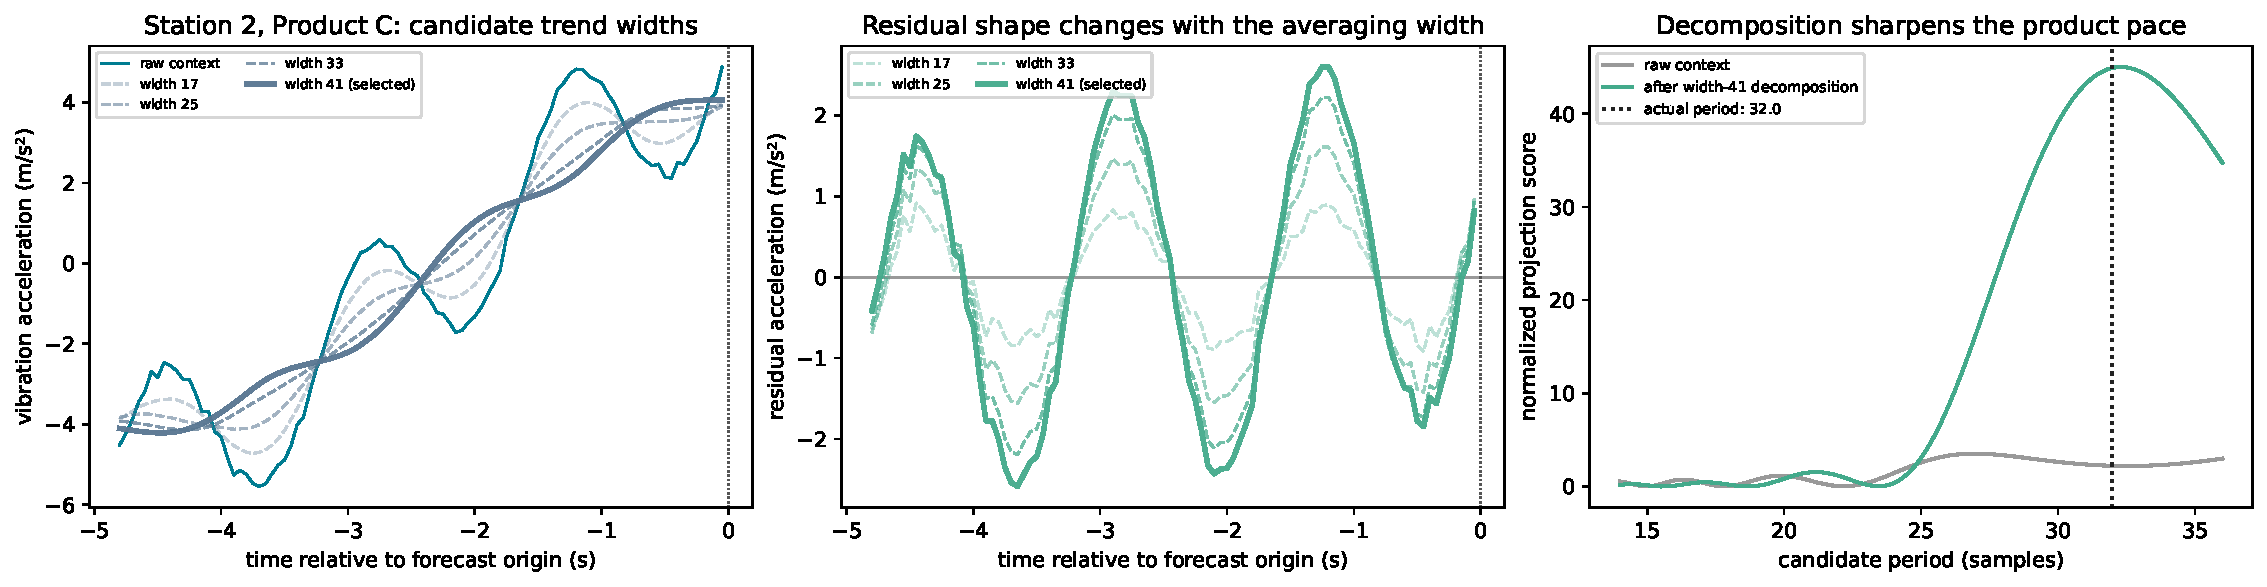
\includegraphics[width=0.85\linewidth]{../Figures/2.1-1.pdf}\caption*{Output 2.1 --- decomposition of one Station 2, Product C context ($P=32$) at widths 17--41}\end{figure}
\textbf{Selected width: $m=41$.} The study selects the width that gives the best oracle period recovery on the training data of Stations 1--3 (Output 2.2).
\begin{itemize}
\item \textbf{Visual change (Output 2.1).} At $m=17$ the trend still follows part of the vibration, so $S$ loses amplitude (residual std 0.58 m/s$^2$). As $m$ grows, $T$ becomes a smooth ramp and $S$ keeps the full cycle (std 1.01, 1.37 and 1.57 m/s$^2$ at 25, 33 and 41). After width-41 decomposition, the period score peaks sharply at the actual period of 32.
\item \textbf{Oracle diagnostic (Output 2.2, training windows).} Recovery within one sample is 0.687 on the raw context, then 0.980, 0.989, 0.993 and 0.998 at widths 17, 25, 33 and 41. There is a trade-off: the median period error is smallest at $m=25$ (0.12 samples, vs 0.22 at $m=41$). The selection rule counts hits within one sample, so $m=41$ wins.
\item \textbf{Ablation (Output 2.3, validation).} Raw Attention 0.466 $\to$ Attention + decomposition 0.310 on Est. ($-33\%$), and 0.679 $\to$ 0.455 on S4 ($-33\%$). Every product improves. The largest gain is S4, Product A (0.731 $\to$ 0.385), and the smallest is S4, Product B (0.617 $\to$ 0.518).
\end{itemize}
\begin{figure}[H]\centering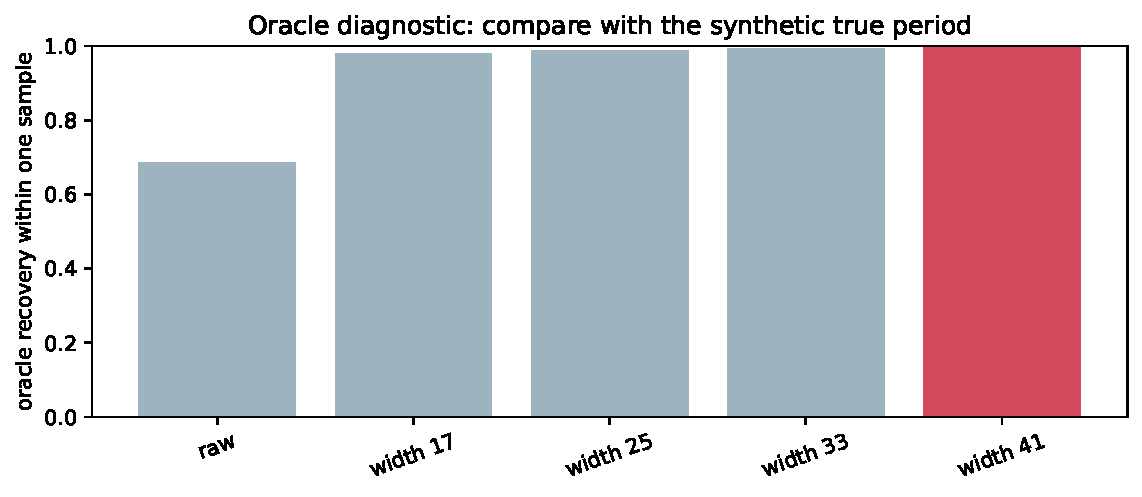
\includegraphics[width=0.75\linewidth]{../Figures/2.2-1.pdf}\caption*{Output 2.2 --- oracle period-recovery diagnostic (training data, Stations 1--3)}\end{figure}
\textbf{Why a moving average fits this world.} Drift (240-sample scale) and vibration (14--36 samples) are well separated in frequency. A moving average whose width spans at least one full cycle ($41>36$) cancels the vibration while still following the slow ramp, because $41\ll240$. It is therefore a cheap low-pass filter with its cutoff between the two components. The oracle diagnostic is a useful selector here because it scores what $S$ actually retains (is the true period recoverable from it?) instead of assuming that $S$ equals $s_i$. It uses only training windows from Stations 1--3, so neither S4 nor the validation and test regions influence $m$. The true period is available only in this synthetic world and is never given to the forecaster.
\begin{figure}[H]\centering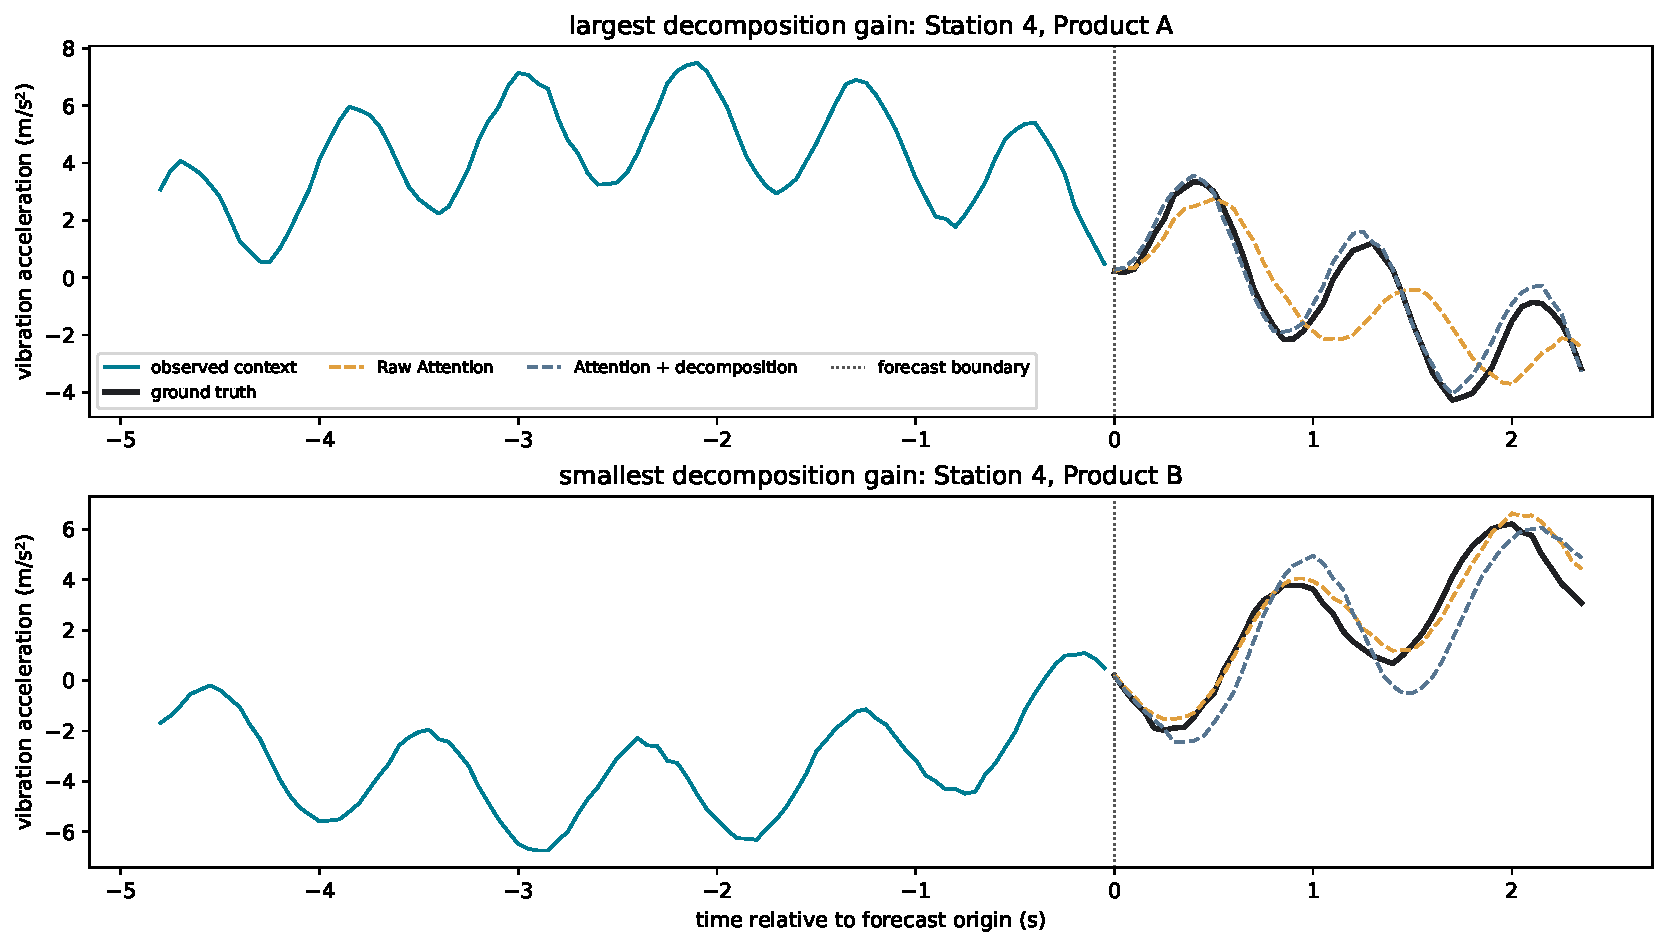
\includegraphics[width=0.75\linewidth]{../Figures/2.3-1.pdf}\caption*{Output 2.3 --- decomposition ablation (largest and smallest gain, S4)}\end{figure}
\textbf{Where it fails:} an abrupt level shift, such as a step in the calibration offset, is smeared into a ramp of width $m$, which leaks a fake trend into $S$ near the step. A wide kernel ($41\approx$ half the 96-sample context) also makes the replicated endpoints affect a large share of the window. \textbf{Alternative:} STL (LOESS) handles curved trends, but it assumes one known, fixed seasonal period. That assumption is wrong here, where pace changes from run to run.

\subsection*{Response 3: Temporal delay mixing}
\texttt{aggregate\_delays} (Eq.~6) builds the source index $(t-\tau_j)\bmod L$ for every example, delay and position. It gathers $v$ at those indices, weights the result by $\alpha_j$ (the same weights for all heads and features of that example), and sums over $j$. On the worked example ($v=[10,20,30,40]$, delays $[1,3]$, weights $[3/4,1/4]$) it returns $[35,15,25,25]$. Because $z_0=35$ (not 25), the shift reads $t-\tau$ in the correct direction. The FFT \texttt{delay\_scores} matches the direct calculation $[4,-4,4,-4]$ (Output 3.1).
\begin{figure}[H]\centering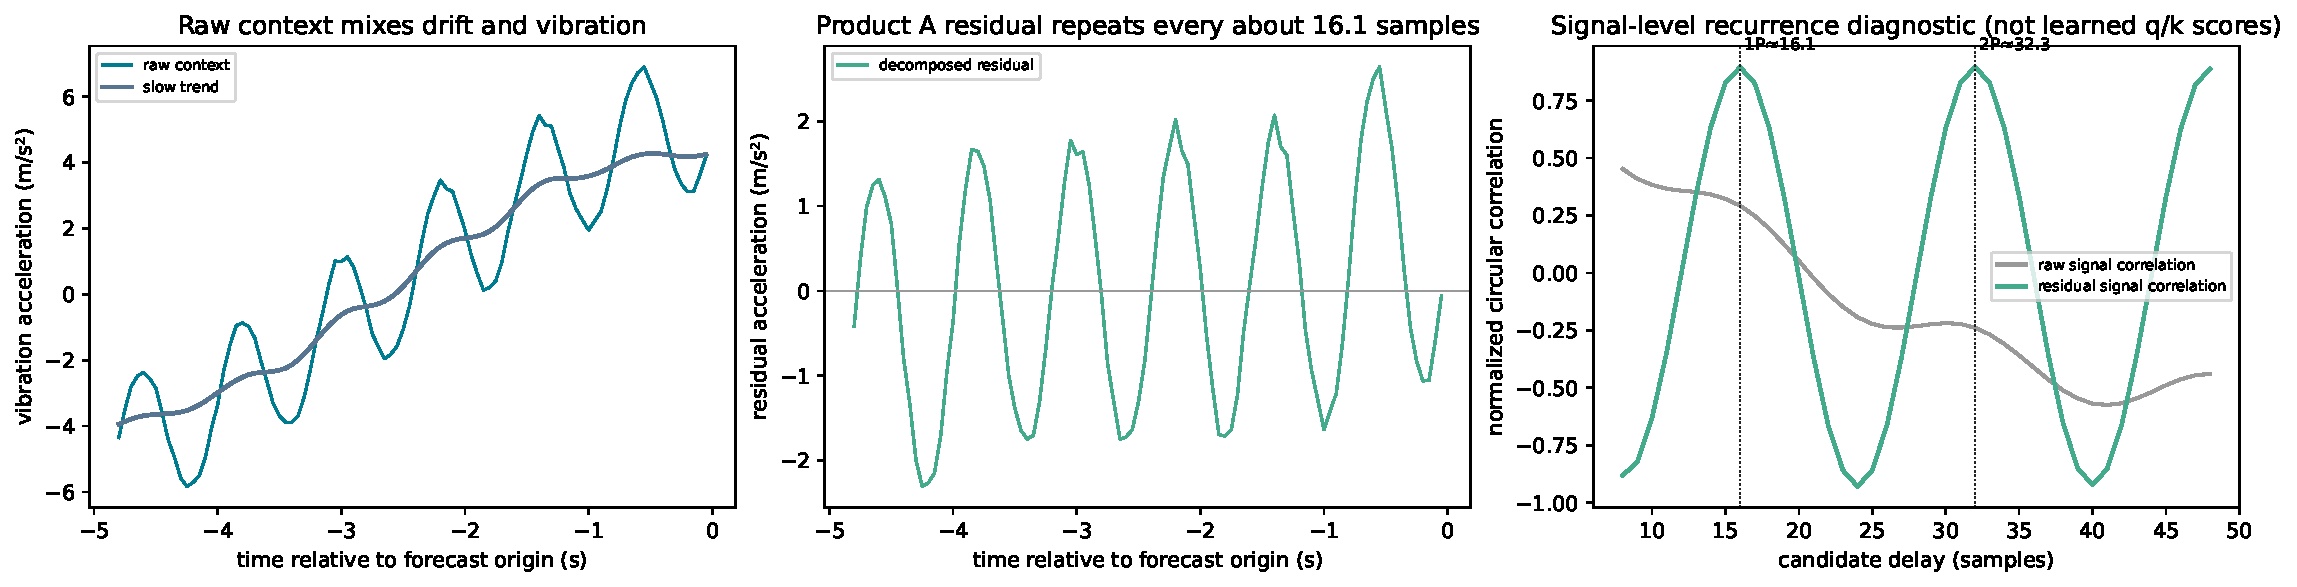
\includegraphics[width=0.85\linewidth]{../Figures/3.2-1.pdf}\caption*{Output 3.2 --- signal-level recurrence diagnostic, Station 2, Product A ($P\approx16.1$)}\end{figure}
\begin{itemize}
\item \textbf{Strongest lags:} the residual correlation peaks at lag 16 ($\approx P=16.1$, correlation 0.896) and at lag 32 ($\approx 2P=32.3$, correlation 0.897). A periodic signal matches itself at every integer multiple of $P$, so the second peak is the same recurrence one cycle further back. 
\item \textbf{Why decomposing first helps:} a ramp stays similar to itself after any shift. In the raw signal the correlation is therefore highest at the shortest lag ($\approx0.45$ at lag 8) and decays smoothly, with only a shallow shoulder near $P$ and no peak at $2P$. Once $T$ is removed, the curve swings between $\approx+0.9$ at $P$ and $2P$ and $\approx-0.9$ at the half-periods, and it rises again towards $3P\approx48$. The delays that matter then stand out, which is exactly the evidence the delay mixer selects with its top-$K$ step. This supports building the delay assumption into the mixer.
\item \textbf{Where the assumption is wrong:} an isolated transient, such as a single impact or shock, has no recurring displacement. Top-$K$ delay selection still picks $K=10$ lags, so the mixer either copies the shock forward at those lags, creating phantom repeats, or averages it away. Attention could instead have treated the transient as a one-off event.
\end{itemize}
\textit{Note: Output 3.2 is a correlation computed directly on the signal. It is not the trained mixer's learned q/k delay scores.}

\subsection*{Response 4: Compare designs and deploy}
\textbf{(a) Prediction (written before Output 4.1).} Decomposition should help most, because it removes the slow ramp before the mixer, so neither Attention nor the delay scores are dominated by drift.

\textbf{(b) Validation results} (Outputs 1.1, 4.1, 4.2).
\begin{table}[H]\centering\small
\begin{tabular}{lcccccr}\toprule
Model & Est. RMSE & Est. MSE & S4 RMSE & S4 MSE & Params & Fit time\\\midrule
Raw Attention & 0.466 & 0.217 & 0.679 & 0.461 & 368,368 & 158 s\\
Attention + decomposition & 0.310 & 0.096 & 0.455 & 0.207 & 373,024 & 455 s\\
Raw delay mixer & 0.215 & 0.046 & 0.341 & 0.116 & 368,370 & 239 s\\
Autoformer-inspired & 0.199 & 0.040 & 0.242 & 0.059 & 373,026 & 510 s\\\midrule
Shared ridge & 0.767 & 0.588 & 0.876 & 0.767 & 4,608 & $<$0.01 s\\
Sensor-specific ridge & 0.768 & 0.590 & n/a & n/a & 13,824 & $<$0.01 s\\
Period-routed ridge & \textbf{0.166} & \textbf{0.028} & \textbf{0.173} & \textbf{0.030} & 59,904 & $<$0.01 s\\\bottomrule
\end{tabular}\end{table}
\begin{figure}[H]\centering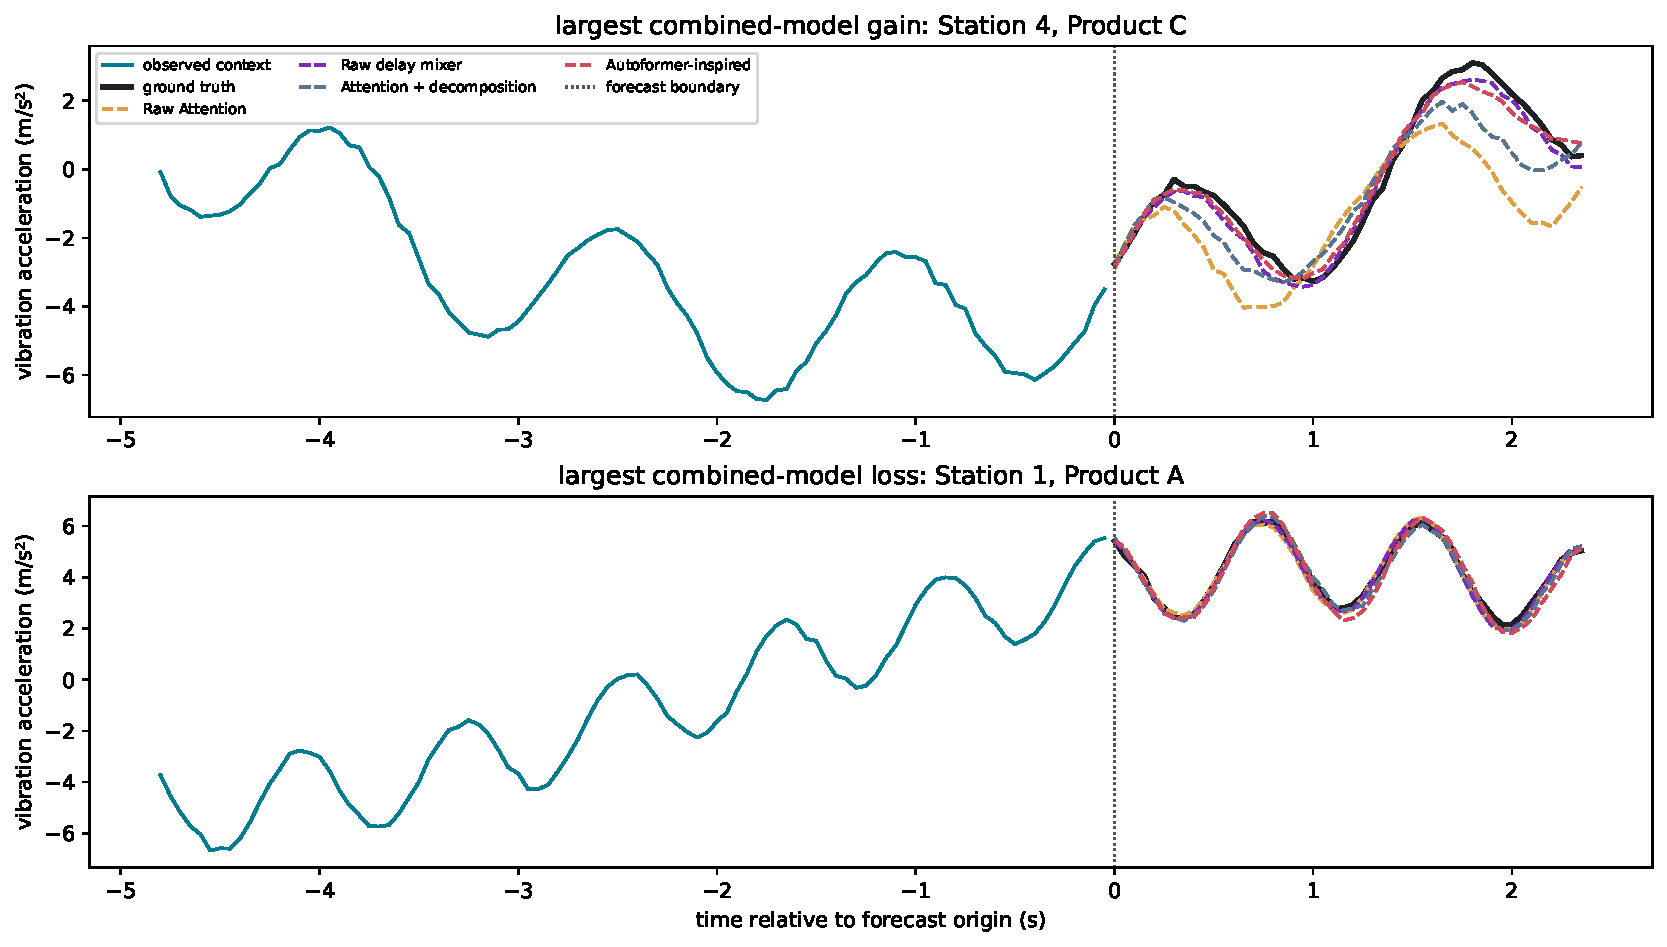
\includegraphics[width=0.85\linewidth]{../Figures/4.1-1.pdf}\caption*{Output 4.1 --- contrasting forecast cases (largest combined-model gain and loss)}\end{figure}
\begin{figure}[H]\centering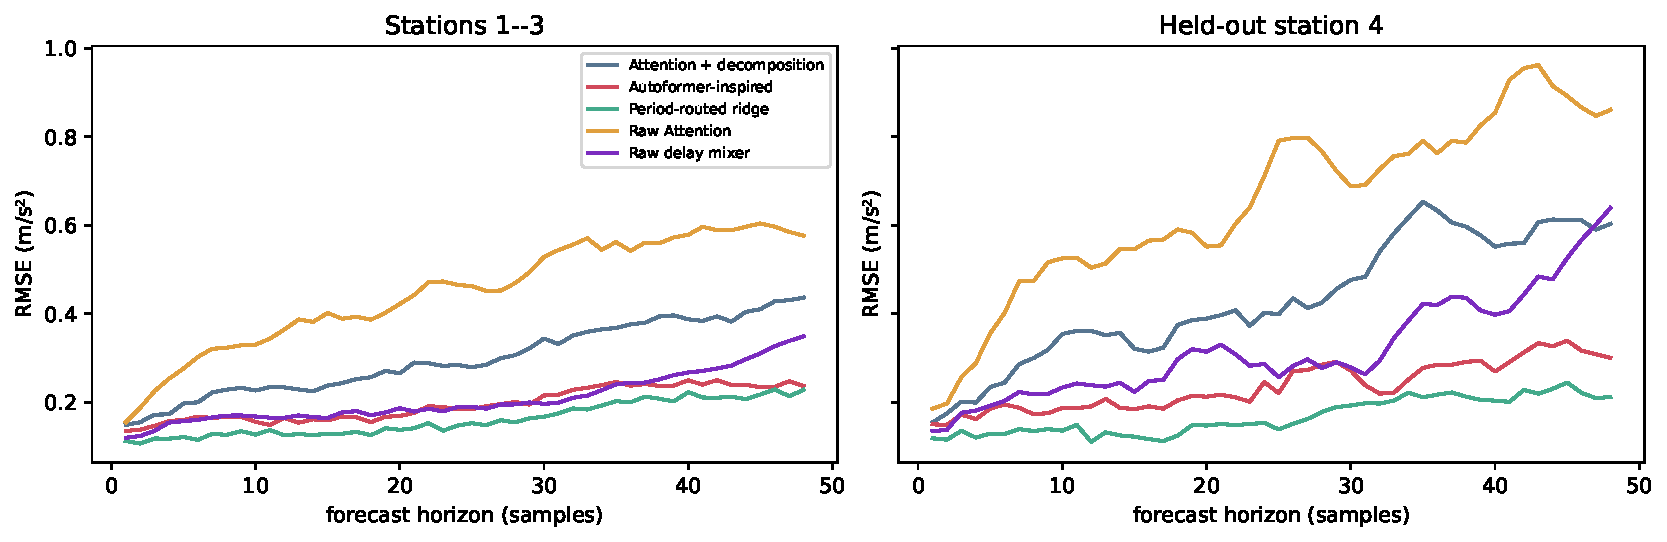
\includegraphics[width=0.75\linewidth]{../Figures/4.2-1.pdf}\caption*{Output 4.2 --- validation RMSE by forecast horizon}\end{figure}
\textbf{Interpretation} (validation; Est.\ / S4 RMSE reduction):
\begin{itemize}
\item \textbf{Delay switch:} $-54\%$ / $-50\%$ with the raw input, and $-36\%$ / $-47\%$ on top of decomposition.
\item \textbf{Decomposition switch:} $-33\%$ / $-33\%$ with Attention, but only $-7\%$ / $-29\%$ on top of the delay mixer.
\item \textbf{Overlap:} combined, $-57\%$ / $-64\%$. Gains are sub-additive (Est.: $0.251+0.156$ vs $0.267$ observed): both switches address the same drift-plus-repetition structure. Contrary to (a), delay mixing gives the larger gain. The combination is not uniformly better (Station 1, Product A is its largest loss, Output 4.1).
\item \textbf{Horizon:} error grows with lead time for all models (first vs last 12 steps): $\times$2.0--2.2 for both Attention models, $\times$1.5 / $\times$1.7 for Autoformer-inspired, and $\times$2.4 on S4 for the raw delay mixer. Period-routed ridge is lowest at all 48 steps.
\end{itemize}

\textbf{(c) Deployment} (chosen in the notebook before Output 4.3 was run).
\begin{itemize}
\item \textbf{Established stations: period-routed ridge.} It has the best validation RMSE/MSE (0.166 / 0.028 vs 0.199 / 0.040 for Autoformer-inspired), 6.2$\times$ fewer parameters, and fits instantly.
\item \textbf{Station 4: period-routed ridge.} It needs only the period estimated from S4's own context, not station identity (0.173 vs 0.242).
\item \textbf{Output 4.3 (test):} 0.161 (Est.) and 0.183 (S4), consistent with validation. The right inductive bias beats flexibility; Autoformer-inspired is the best \emph{learned} model.
\end{itemize}
